%%%%%%%%%%%%%%%%%%%%%%%%%%%%%%%%%%%%%%%%%%%%%%%%%%%
%                                                 %
%                     SECTION                     %
%                                                 %
%%%%%%%%%%%%%%%%%%%%%%%%%%%%%%%%%%%%%%%%%%%%%%%%%%%

\section{Description}
\label{sec:sec003}

To verify our work, we identified measurable and explicit targets. By having several goals, including that a value percentage of the users should be able to operate the tasks without the need of help. On the same rate value, the user should be able to start and complete the medical diagnosis tasks over the system with little errors or mitigating those errors. Measuring the expected number of errors with a relation between our laboratory pilot tests. On the laboratory pilot tests we aim to test our prototypes with researchers. The Researchers are in the context of the system and know well the functionalities so that we need to expect a percentage value over their results compared to clinicians and not the same benefits. Last but not least, both users (researchers and clinicians) should be able to understand in a similar time amount the meaning of all visible controls. By the similar amount of time, it is expected to have a variance of the percentage value between researchers and clinicians of the same value percentage of the early goals described in this paragraph.

We tested each objective in early laboratory and field tests so that we could take the appropriate corrective actions. Also, we expect to run early field tests with researchers and clinicians to highlight issues that we overlooked and ignored during the prototyping phase. To support interaction use by the clinicians, we will try to emphasise several key factors on our user tests. The tasks must be simple, low intrusive, support for natural interaction and the system must always give visibility and the task current-state.

\clearpage

%%%%%%%%%%%%%%%%%%%%%%%%%%%%%%%%%%%%%%%%%%%%%%%%%%%
%                                                 %
%                     SECTION                     %
%                                                 %
%%%%%%%%%%%%%%%%%%%%%%%%%%%%%%%%%%%%%%%%%%%%%%%%%%%

\subsection{Devices}

Traditional interaction remains the most common way to interact with user interfaces in a clinical environment. Unfortunately, most of this interaction is made by low profile equipment that makes users produce more errors and take more time interacting with those user interfaces.

On Figure \ref{fig:patient_list} the user can select the list of patients. The list has a table with several patient information. The first column is the \textit{Patient ID}; we used it as an identifier of the patient. That way we can have anonymised information with no reference to the patient name. The second column is the \textit{Study Date}, the third column is the \textit{Modality} of the used \textbf{DICOM} image, the fourth column is the \textit{Study Description} of the used study and the last column is the number of \textit{Images}.

%%%%%%%%%%%%%%%%%%%%%%%%%%%%%%%%%%%%%%%%%%%%%%%%%%%

\hfill

\begin{figure}[h]
\centering
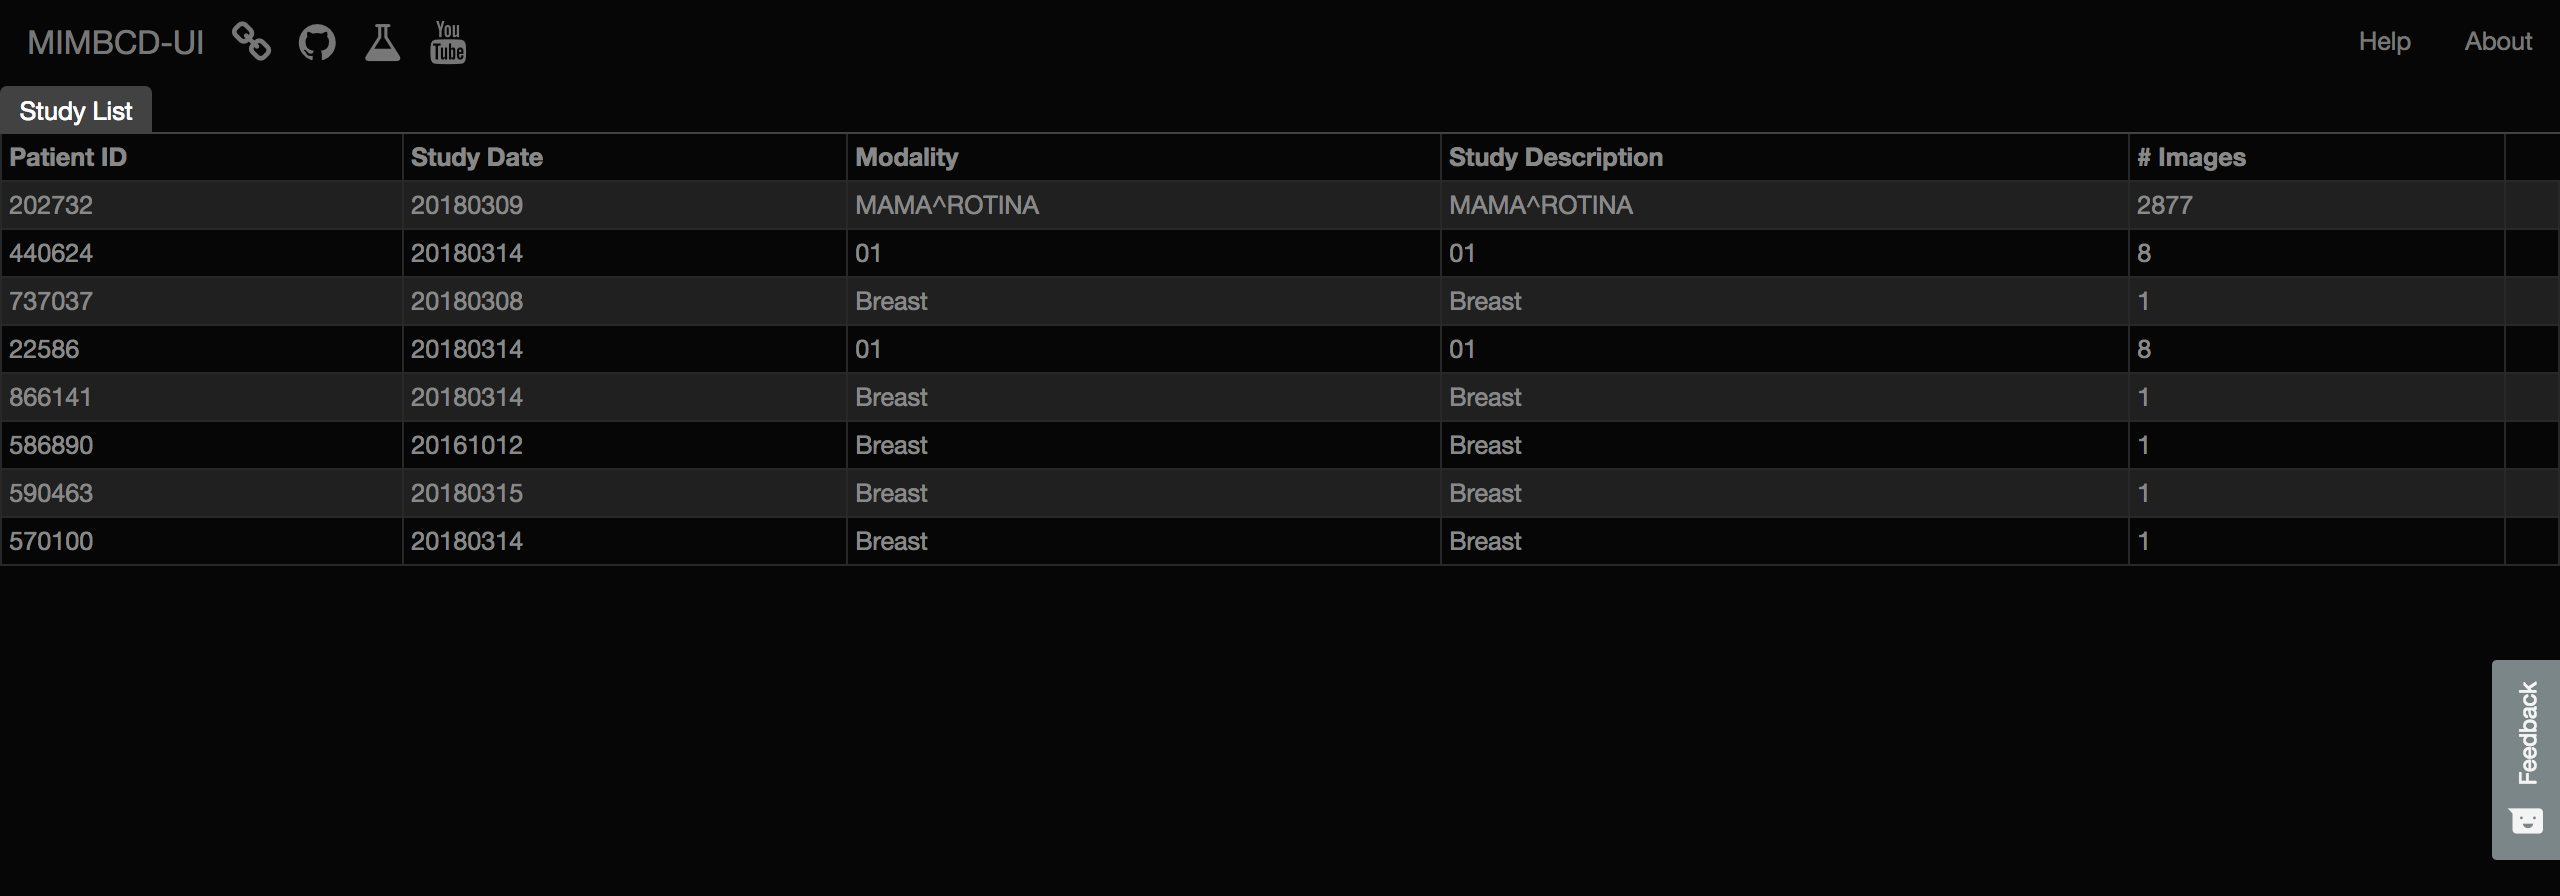
\includegraphics[width=\textwidth]{patient_list}
\caption{List of Patients.}
\label{fig:patient_list}
\end{figure}

\hfill

%%%%%%%%%%%%%%%%%%%%%%%%%%%%%%%%%%%%%%%%%%%%%%%%%%%

As we can see in Figure \ref{fig:image_viewer}, it shows the first task in our User Interface (UI), where the patient's breasts are on a small left column. The options are in a short row near of the viewport and described below. We also have the tabs where the user can change the patient. The centre viewport shows the \textbf{DICOM} image, and it can be configured to display a number up to four \textbf{DICOM} images at the same time. The viewport has some text information on it (yellow) with the details of the metadata. Nevertheless, the \textbf{Assistant} suggestions are shown on the top-right corner of the system.

\clearpage

%%%%%%%%%%%%%%%%%%%%%%%%%%%%%%%%%%%%%%%%%%%%%%%%%%%

\hfill

\begin{figure}[h]
\centering
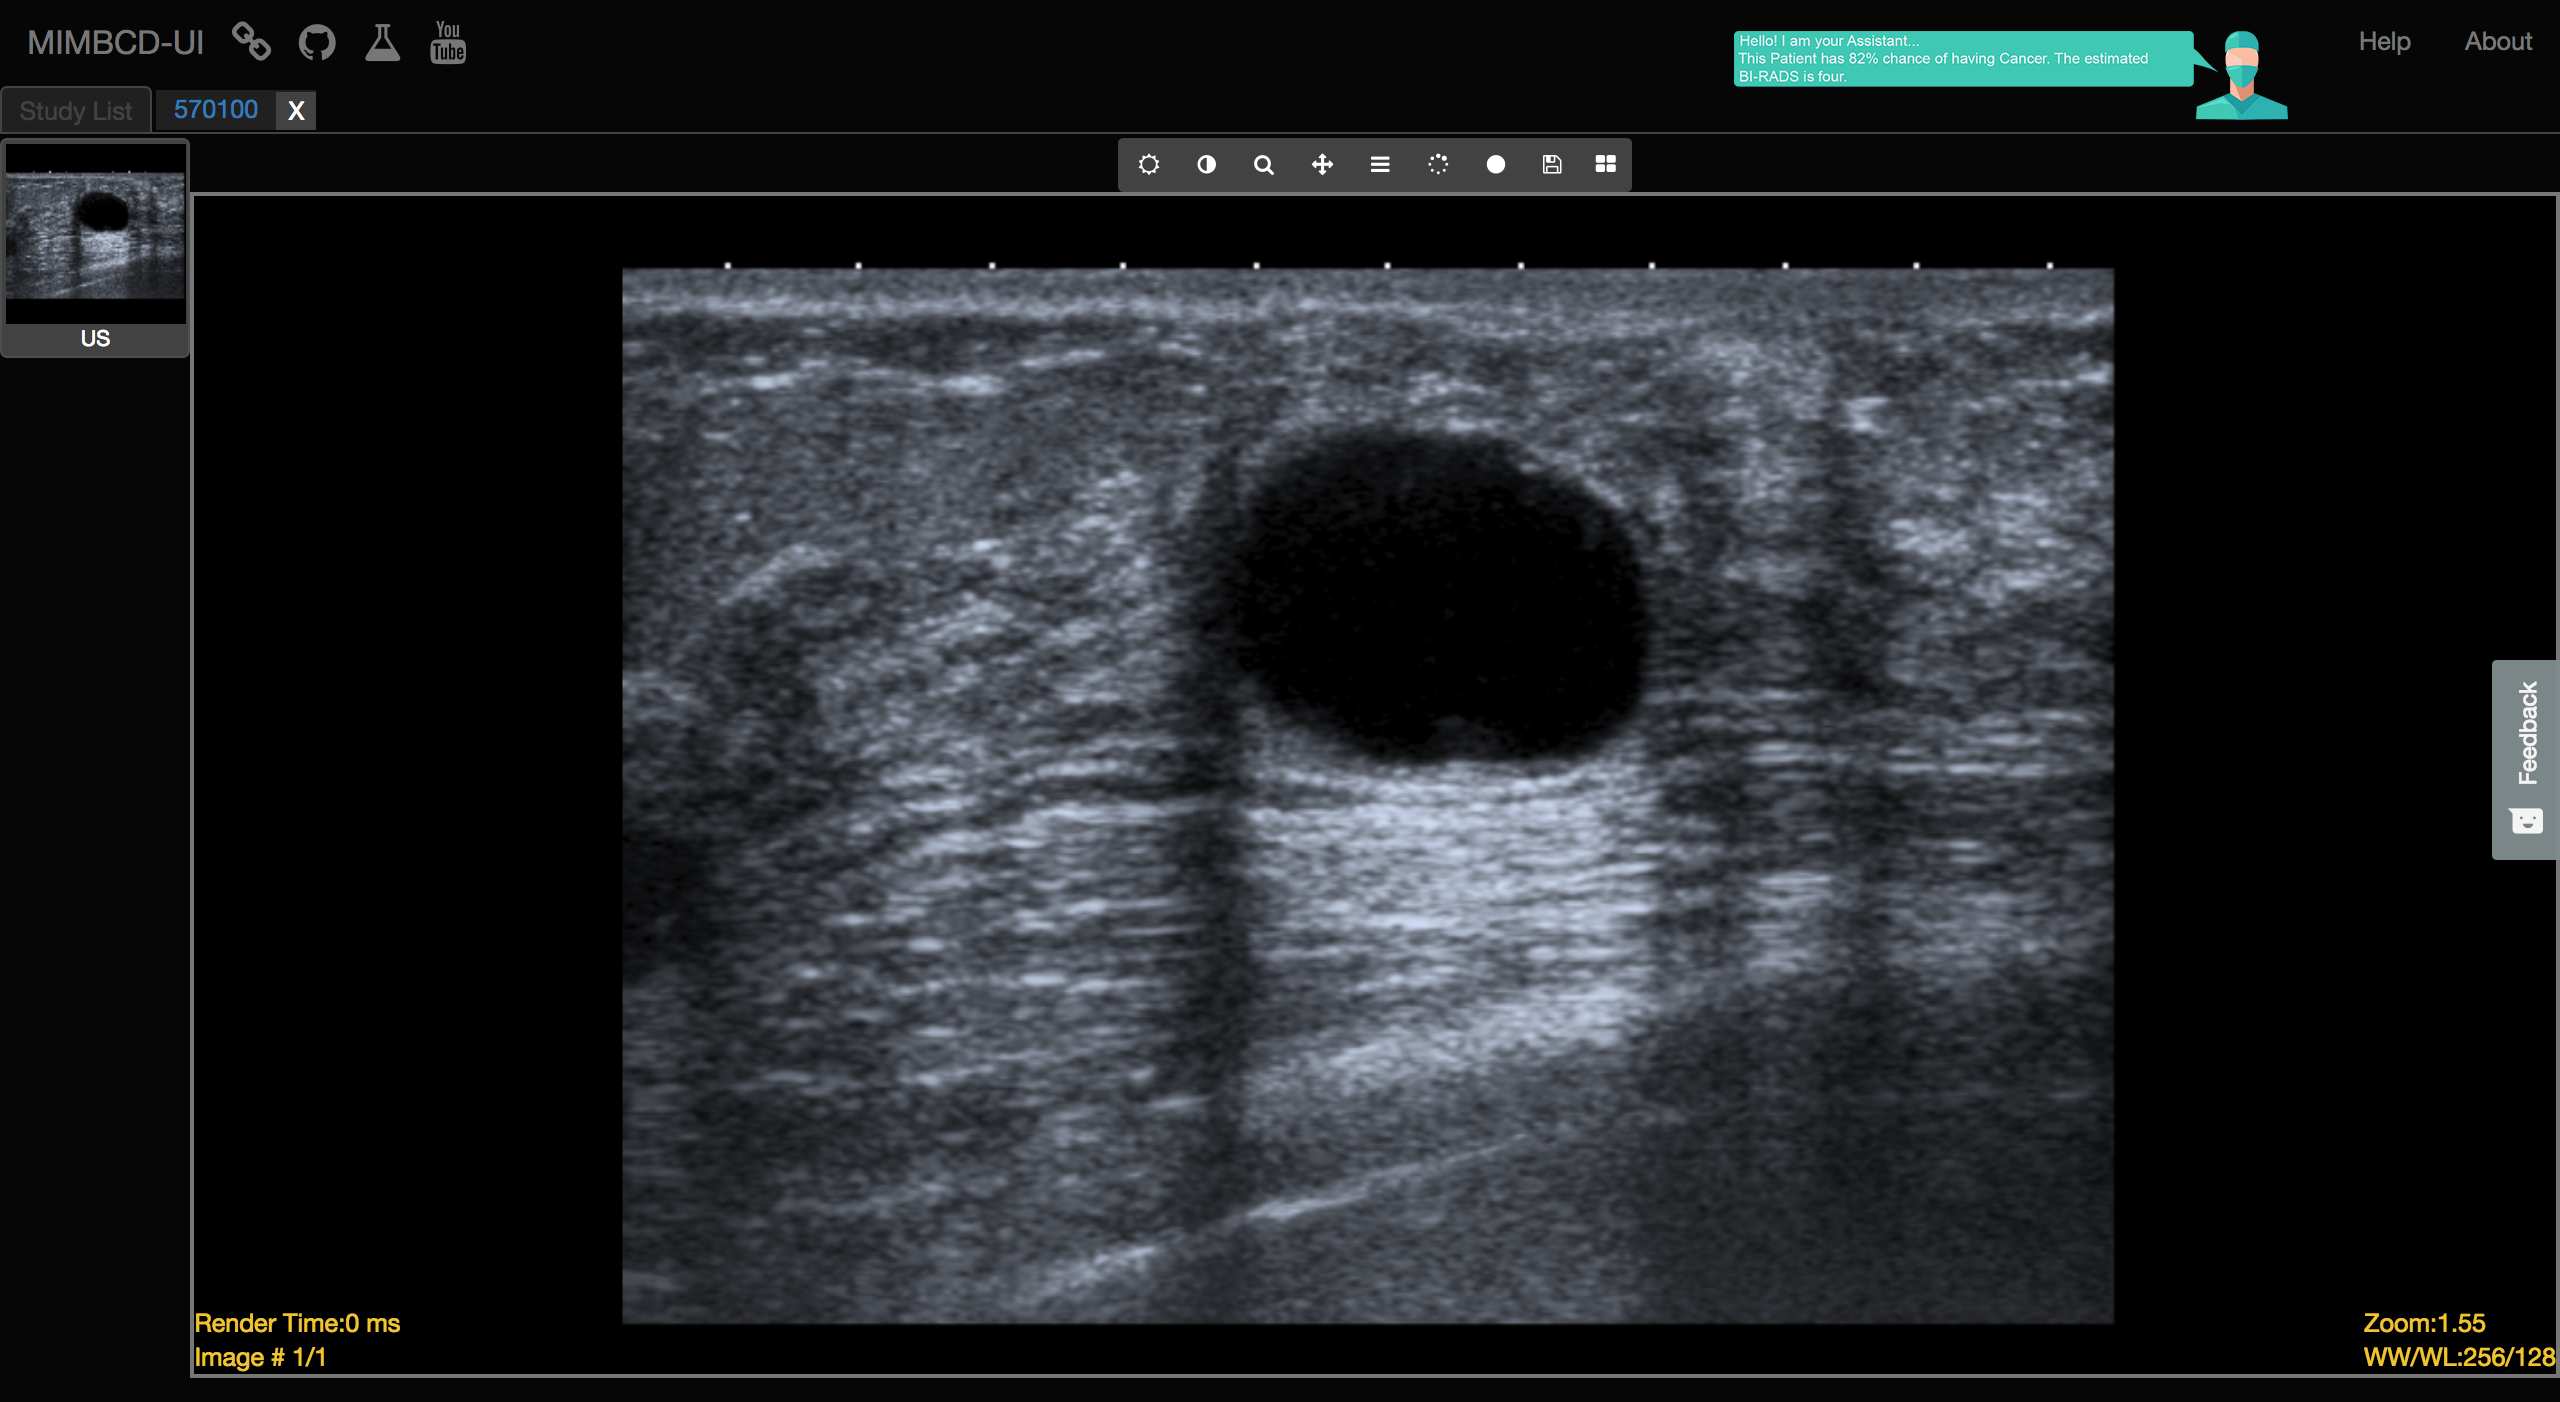
\includegraphics[width=\textwidth]{image_viewer}
\caption{Viewer of the \textbf{DICOM} images.}
\label{fig:image_viewer}
\end{figure}

\hfill

%%%%%%%%%%%%%%%%%%%%%%%%%%%%%%%%%%%%%%%%%%%%%%%%%%%

Manual annotation is adopted by us thanks to Freehand ROI and Probe annotation features, both from \hyperlink{https://cornerstonejs.org/}{CornerstoneJS}. According to the \hyperlink{https://cornerstonejs.org/}{CornerstoneJS} Library, the user can create an annotation by setting up consecutive landmarks around a Region of Interest (ROI). The markers finish a lesion annotation when it interconnects the historical. Additional features available in our User Interface (UI) includes on-demand increment of the number of landmarks, and throw transformations of the shape of an annotation.

\clearpage

%%%%%%%%%%%%%%%%%%%%%%%%%%%%%%%%%%%%%%%%%%%%%%%%%%%
%                                                 %
%                     SECTION                     %
%                                                 %
%%%%%%%%%%%%%%%%%%%%%%%%%%%%%%%%%%%%%%%%%%%%%%%%%%%

\subsection{User Interactions}

The systems have several buttons (Figure \ref{fig:toolbar}) that allows the user to interact or access to a set of user interface features. Each item of the following list represents each metaphoric icon of Figure \ref{fig:toolbar}.

%%%%%%%%%%%%%%%%%%%%%%%%%%%%%%%%%%%%%%%%%%%%%%%%%%%

\hfill

\begin{figure}[h]
\centering

\includegraphics[width=\textwidth]{toolbar}
\caption{Toolbar of the System available features.}
\label{fig:toolbar}
\end{figure}

\hfill

%%%%%%%%%%%%%%%%%%%%%%%%%%%%%%%%%%%%%%%%%%%%%%%%%%%

\hfill

The buttons are (from left to right of Figure \ref{fig:toolbar}) as follows:

\hfill

\begin{itemize}
\item WW/WC
\item Invert
\item Zoom
\item Pan
\item Stack Scroll
\item Freehand
\item Probe
\item Save
\item Window Controller
\end{itemize}

\hfill

\clearpage

%%%%%%%%%%%%%%%%%%%%%%%%%%%%%%%%%%%%%%%%%%%%%%%%%%%
%                                                 %
%                     SECTION                     %
%                                                 %
%%%%%%%%%%%%%%%%%%%%%%%%%%%%%%%%%%%%%%%%%%%%%%%%%%%

\subsection{Evaluation}

Introduction of AI \textbf{Assistant} agents are significant factors which can naturally affect the performance of a medical workflow. While some prior studies \cite{Calisto:2017:TTM:3132272.3134111} have investigated the functionality of healthcare systems, the \textit{AI-Assisted} acceptability has mostly been overlooked in the existing Health Informatics (HI) literature regarding a Human-Computer Interaction (HCI).

The following Table \ref{table:usability_evaluation_questions} is presenting seven evaluation questions to have in mind during evaluation. The purpose of this questions is to facilitate systematic user studies regarding our novel \textbf{Assistant} in a clinical environment and support user stimulation for the introduction of \textit{AI-Assisted} methods. The proposed issues involve various aspects of workflow combined with either need for satisfaction or division of attention.

\hfill

\begin{table}[h]
\centering
\begin{tabular}{l|l}
Number & Issues of Content \& Key Questions                    	 \\ \hline
1      & How would the user describe the potential adoption of   \\
       & \textit{AI-Assisted} methods on the Health Institution? \\ \hline
2      & What are the user oppositions for \textit{AI-Assisted}	 \\
       & methods?                                                \\ \hline
3      & What examples of \textit{AI-Assisted} methods does the  \\
       & user know regarding the Health Institution?             \\ \hline
4      & What are the obstacles of the user's Health             \\
       & Institution?                                            \\ \hline
5      & What is more important for the \textit{AI-Assisted}     \\
       & information, the BIRADS or Pathology?                   \\ \hline
6      & Is it important for the user to have the feature of		 \\
       & Approve, Reject and Justify options?                    \\ \hline
7      & For the user's opinion, what are the aspects that       \\
       & influence the decision?                                 \\ \hline

\end{tabular}
\caption{Usability Evaluation Questions}
\label{table:usability_evaluation_questions}
\end{table}

\hfill

The influence of \textit{AI-Assisted}~\cite{goodfellow2016deep} is an important variable for our empirical analysis. In fact, the trust of the user increases when the user perceived that the \textbf{Assistant} is giving the right inputs and that there will be a consequent increase of the clinician trust in our system.

\clearpage

The first question, the \textit{How would the user describe the potential adoption of \textit{AI-Assisted} methods on the Health Institution?} question. For the second question, the \textit{What are the user oppositions for \textit{AI-Assisted} methods?} question, we aim to understand what are the user constrains regarding an AI adoption the the user's current workflow. Third, we intend to filter possible examples of the clinical applications of AI on the Health Institutions by asking \textit{What examples of \textit{AI-Assisted} methods does the user know regarding the Health Institution?} directly to the clinician. The fourth question, underlines the reasons why several obstacles are present on the Health Institution, with the question \textit{What are the obstacles of the user's Health Institution?} we can understand the challenges of achieving those issues and what are the solutions for surpass it. On the fifth question, where we ask \textit{What is more important for the \textit{AI-Assisted} information, the BIRADS or Pathology?}, we aim to understand what is more important for the user, the BIRADS or the Pathology of the patient~\cite{elverici2015nonpalpable}. Almost last, the six question, where we ask for \textit{Is it important for the user to have the feature of \textbf{Approve}, \textbf{Reject} and \textbf{Justify} options?} is an important question to understand the feature needs and options. Last but not least, the seven question, \textit{For the user's opinion, what are the aspects that influence the decision?}, is where we will understand what is the most important information to show to the clinicians, therefore, we can more effectively and efficiently give more accurate information to the users.

To conclude this section, by doing this questions, we aim to support our user studies by giving our users, the clinicians, the opportunity of improving our empirical analysis regarding user's \textit{open answers}. However, the results should be treated with caution. Several bias exists since we are doing here an ambiguous approach.

\clearpage